\chapter{Lecture 32 - Laplace Equation in Cylindrical Coordinates}
\label{ch:lec32}
\section{Objectives}
\begin{itemize}
\item Solve the steady-state heat equation (Laplace Equation) in cylindrical coordinates for two cases.
\item Re-introduce modified Bessel functions of the first and second kind.
\end{itemize}
\setcounter{lstannotation}{0}

\section{Steady-State Temperature in a Circular Cylinder - Case I}
Consider the boundary value problem below based on the steady-state heat equation in cylindrical coordinates. A schematic of the problem is shown in Figure \ref{fig:lec32-ex1-schematic}.
\begin{table}[h]
\begin{tabular}{l l}
$\substack{\text{Governing} \\\text{Equation}}: $& $\frac{\partial^2 u}{\partial r^2} + \frac{1}{r}\frac{\partial u}{\partial r} + \frac{\partial^2 u}{\partial z^2} + \frac{1}{r^2}\frac{\partial^2 u}{\partial \theta^2}= 0, \ \ \substack{0<r<2, \ \ 0<z<4 \\ \\ 0<\theta<2 \pi}$\\
& \\
$\substack{\text{Boundary} \\ \text{Conditions}}: $ & $u(r,0) = 0, \ u(r,4) = u_0, \ u(2,z) = 0$  \\ 
\end{tabular}
\end{table} 
\begin{marginfigure}
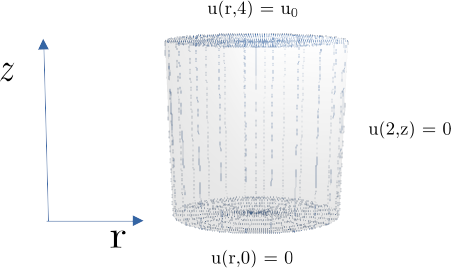
\includegraphics{lec32-ex1-schematic.png}
\caption{Schematic of Case I}
\label{fig:lec32-ex1-schematic}
\end{marginfigure}

\vspace{0.25cm}

\noindent Based on the boundary conditions provided for the problem---none of which are dependent on $\theta$---we can expect that the solution also will be independent of $\theta$ and so the governing equation can be simplified to:
\begin{equation*}
\frac{\partial^2 u}{\partial r^2} + \frac{1}{r}\frac{\partial u}{\partial r} + \frac{\partial^2 u}{\partial z^2} = 0
\end{equation*}

\newthought{As is becoming the usual}, we will solve this problem using separation of variables.

\vspace{0.25cm}

\noindent\textbf{Step \#1:} Assume a product solution:
\begin{equation*}
u(r,z) = F(r)G(z)
\end{equation*}

\vspace{5.0cm}

\noindent\textbf{Step \#2:} Insert the product solution into the governing equation.

\begin{align*}
\frac{\partial^2}{\partial r^2}\left(F(r)G(z) \right) + \frac{1}{r}\frac{\partial}{\partial r}\left(F(r) G(z)\right) + \frac{\partial^2}{\partial z^2}\left( F(r)G(z)\right) &= 0 \\
F_{rr}G + \frac{1}{r}F_rG + FG_{zz} &= 0
\end{align*}

\vspace{0.25cm}

\noindent\textbf{Step \#3:} Separate the variables.

\begin{align*}
\frac{F_{rr}G}{FG} + \frac{1}{r}\frac{F_r G}{FG} + \frac{FG_{zz}}{FG} &= 0 \\
\frac{F_{rr}}{F} + \frac{1}{r}\frac{F_r}{F} + \frac{G_{zz}}{G} &= 0 \\
\frac{F_{rr}}{F} + \frac{1}{r}\frac{F_r}{F} = -\frac{G_{zz}}{G} &= -\lambda
\end{align*}
So the separated equations are:\marginnote{Again, here we multiply the equation for $F(r)$ by $r^2$ to render the equation into a familiar form.}
\begin{align*}
r^2F_{rr} + rF_r + \lambda r^2 F &= 0 \\
G_{zz} - \lambda G &= 0
\end{align*}




